%
%  Scott Percic
%
\documentclass[12pt,fullpage]{article}
\usepackage{fullpage}
\usepackage{psfrag}                                          % LaTeX graphics tool
\usepackage{pslatex}                                         % avoids the default cmr font
\usepackage{graphicx}                                        % graphics package 
\usepackage{epsfig}                                          % figures
\usepackage{hyperref}
\usepackage{color}

\begin{document}

\noindent
{\bf Erlang Distribution} (from \color{blue}\url{http://www.math.wm.edu/~leemis/chart/UDR/UDR.html}\color{black})

\noindent
The shorthand $X \sim {\rm Erlang}(n,\alpha)$ is used to indicate that the
random variable $X$ has the Erlang distribution with positive shape parameter $n$ and positive scale parameter $\alpha$.
An Erlang random variable $X$ with rate $\alpha$ and $n$ stages has probability density function 
$$
f(x) =\frac{x ^ {n - 1} e ^ {-x / \alpha}} {\alpha ^ {n} (n - 1) !} \qquad \qquad x > 0.
$$
The Erlang distribution can be used to model the time to complete $n$ operations
in series, where each operation requires an exponential period of time to complete.
The probability density function for various values of $n$ and $\alpha$ is
%  is $n = 1, 2, 3$ and $\alpha = 1$ is
illustrated below.

\begin{figure}[h!]
\begin{center}
\psfrag{lab1}{$n \kern -0.04 em = \kern -0.04 em 1,\  \alpha \kern -0.04 em = \kern -0.04 em 1$}
\psfrag{lab2}{$n \kern -0.04 em = \kern -0.04 em 3,\  \alpha \kern -0.04 em = \kern -0.04 em 1$}
\psfrag{lab3}{$n \kern -0.04 em = \kern -0.04 em 1,\  \alpha \kern -0.04 em = \kern -0.04 em 4$}
\psfrag{labx}{$x$}
\psfrag{labf}{$f(x)$}
\includegraphics[width=3.2in]{ErlangPlot.ps}
\end{center}
\end{figure}

\noindent
The cumulative distribution function on the support of $X$ is
$$
F(x) = P(X \le x) =1 - \sum_{i = 0} ^ {n - 1} \frac{e ^ {-x / \alpha} \kern 0.08 em x ^ {\kern 0.04 em i}} {\alpha ^ {i} i!}
$$
The survivor function on the support of $X$ is
$$
S(x) = P(X \ge x) =\sum_{i=0}^{n-1}\frac{e^{-x / \alpha}\kern 0.08 em x ^ {\kern 0.04 em i}} {\alpha ^ {i} i!} \qquad \qquad x > 0.
$$
The hazard function on the support of $X$ is
$$
h(x) = \frac{f(x)}{S(x)} =
\frac{x ^ {n - 1}}{\alpha ^ n (n - 1)! \sum_{i=0}^{n-1} x ^ {\kern 0.04 em i}/(\alpha ^ {i} i!)}
\qquad \qquad x > 0.
$$
The cumulative hazard function of $X$ is $H(x) = -\ln S(x)$ is not mathematically tractable. 
The inverse distribution function of $X$ is also intractable,
although random variates can be generated via
$$
X \leftarrow - \alpha \ln \left( \prod_{i\,=\,1}^n U_i \right),
$$
where $U_1, U_2, \ldots, U_n$ are independent and identically distributed $U(0, 1)$ random variates.
There is no closed-form expression for the median.
The moment generating function of $X$ is
$$
M(t) = E\left[ e ^ {tX} \right] = \left( 1 - \alpha t \right) ^ {-n} \qquad \qquad t \le \alpha.
$$
The characteristic function of $X$ is
$$
\phi(t) = E\left[ e ^ {itX} \right] = (1 - i \alpha t) ^ {-n}  \qquad \qquad t < \alpha.
$$
The population mean, variance, skewness, and kurtosis of $X$ are
$$
E[X] = n \alpha \qquad \qquad 
V[X] = n \alpha ^ {2} \qquad \qquad 
E\left[ \left( \frac{X - \mu}{\sigma} \right) ^ 3 \right] = \frac{2}{\sqrt{n}} \qquad \qquad 
E\left[ \left( \frac{X - \mu}{\sigma} \right) ^ 4 \right] = 3 +\frac{6}{n}.
$$

\vspace{0.1in}

\noindent
{\bf APPL verification:}
The APPL statements
\begin{verbatim}
assume(n, posint);
assume(alpha > 0);
X:=[[x -> x ^ (n - 1) * exp(-x / alpha) / (alpha ^ n * (n-1)!)], [0, infinity],
    ["Continuous", "PDF"]];
CDF(X);
HF(X);
CHF(X);
Mean(X);
Variance(X);
Skewness(X);
Kurtosis(X);
MGF(X);
\end{verbatim}
verify the cumulative distribution function, hazard function, cumulative hazard function, population mean, variance, skewness, kurtosis, and moment generating function.
\end{document}
